\subsection{Drivetrain}
The drivetrain of a motorized vehicle, is the components that transfer the rotational energy from the motor to the drive wheel of the vehicle. To understand the function of the different components, a picture of the vehicle can be seen on \figref{FullVehicle}. 

\begin{figure}[H]
	\centering
	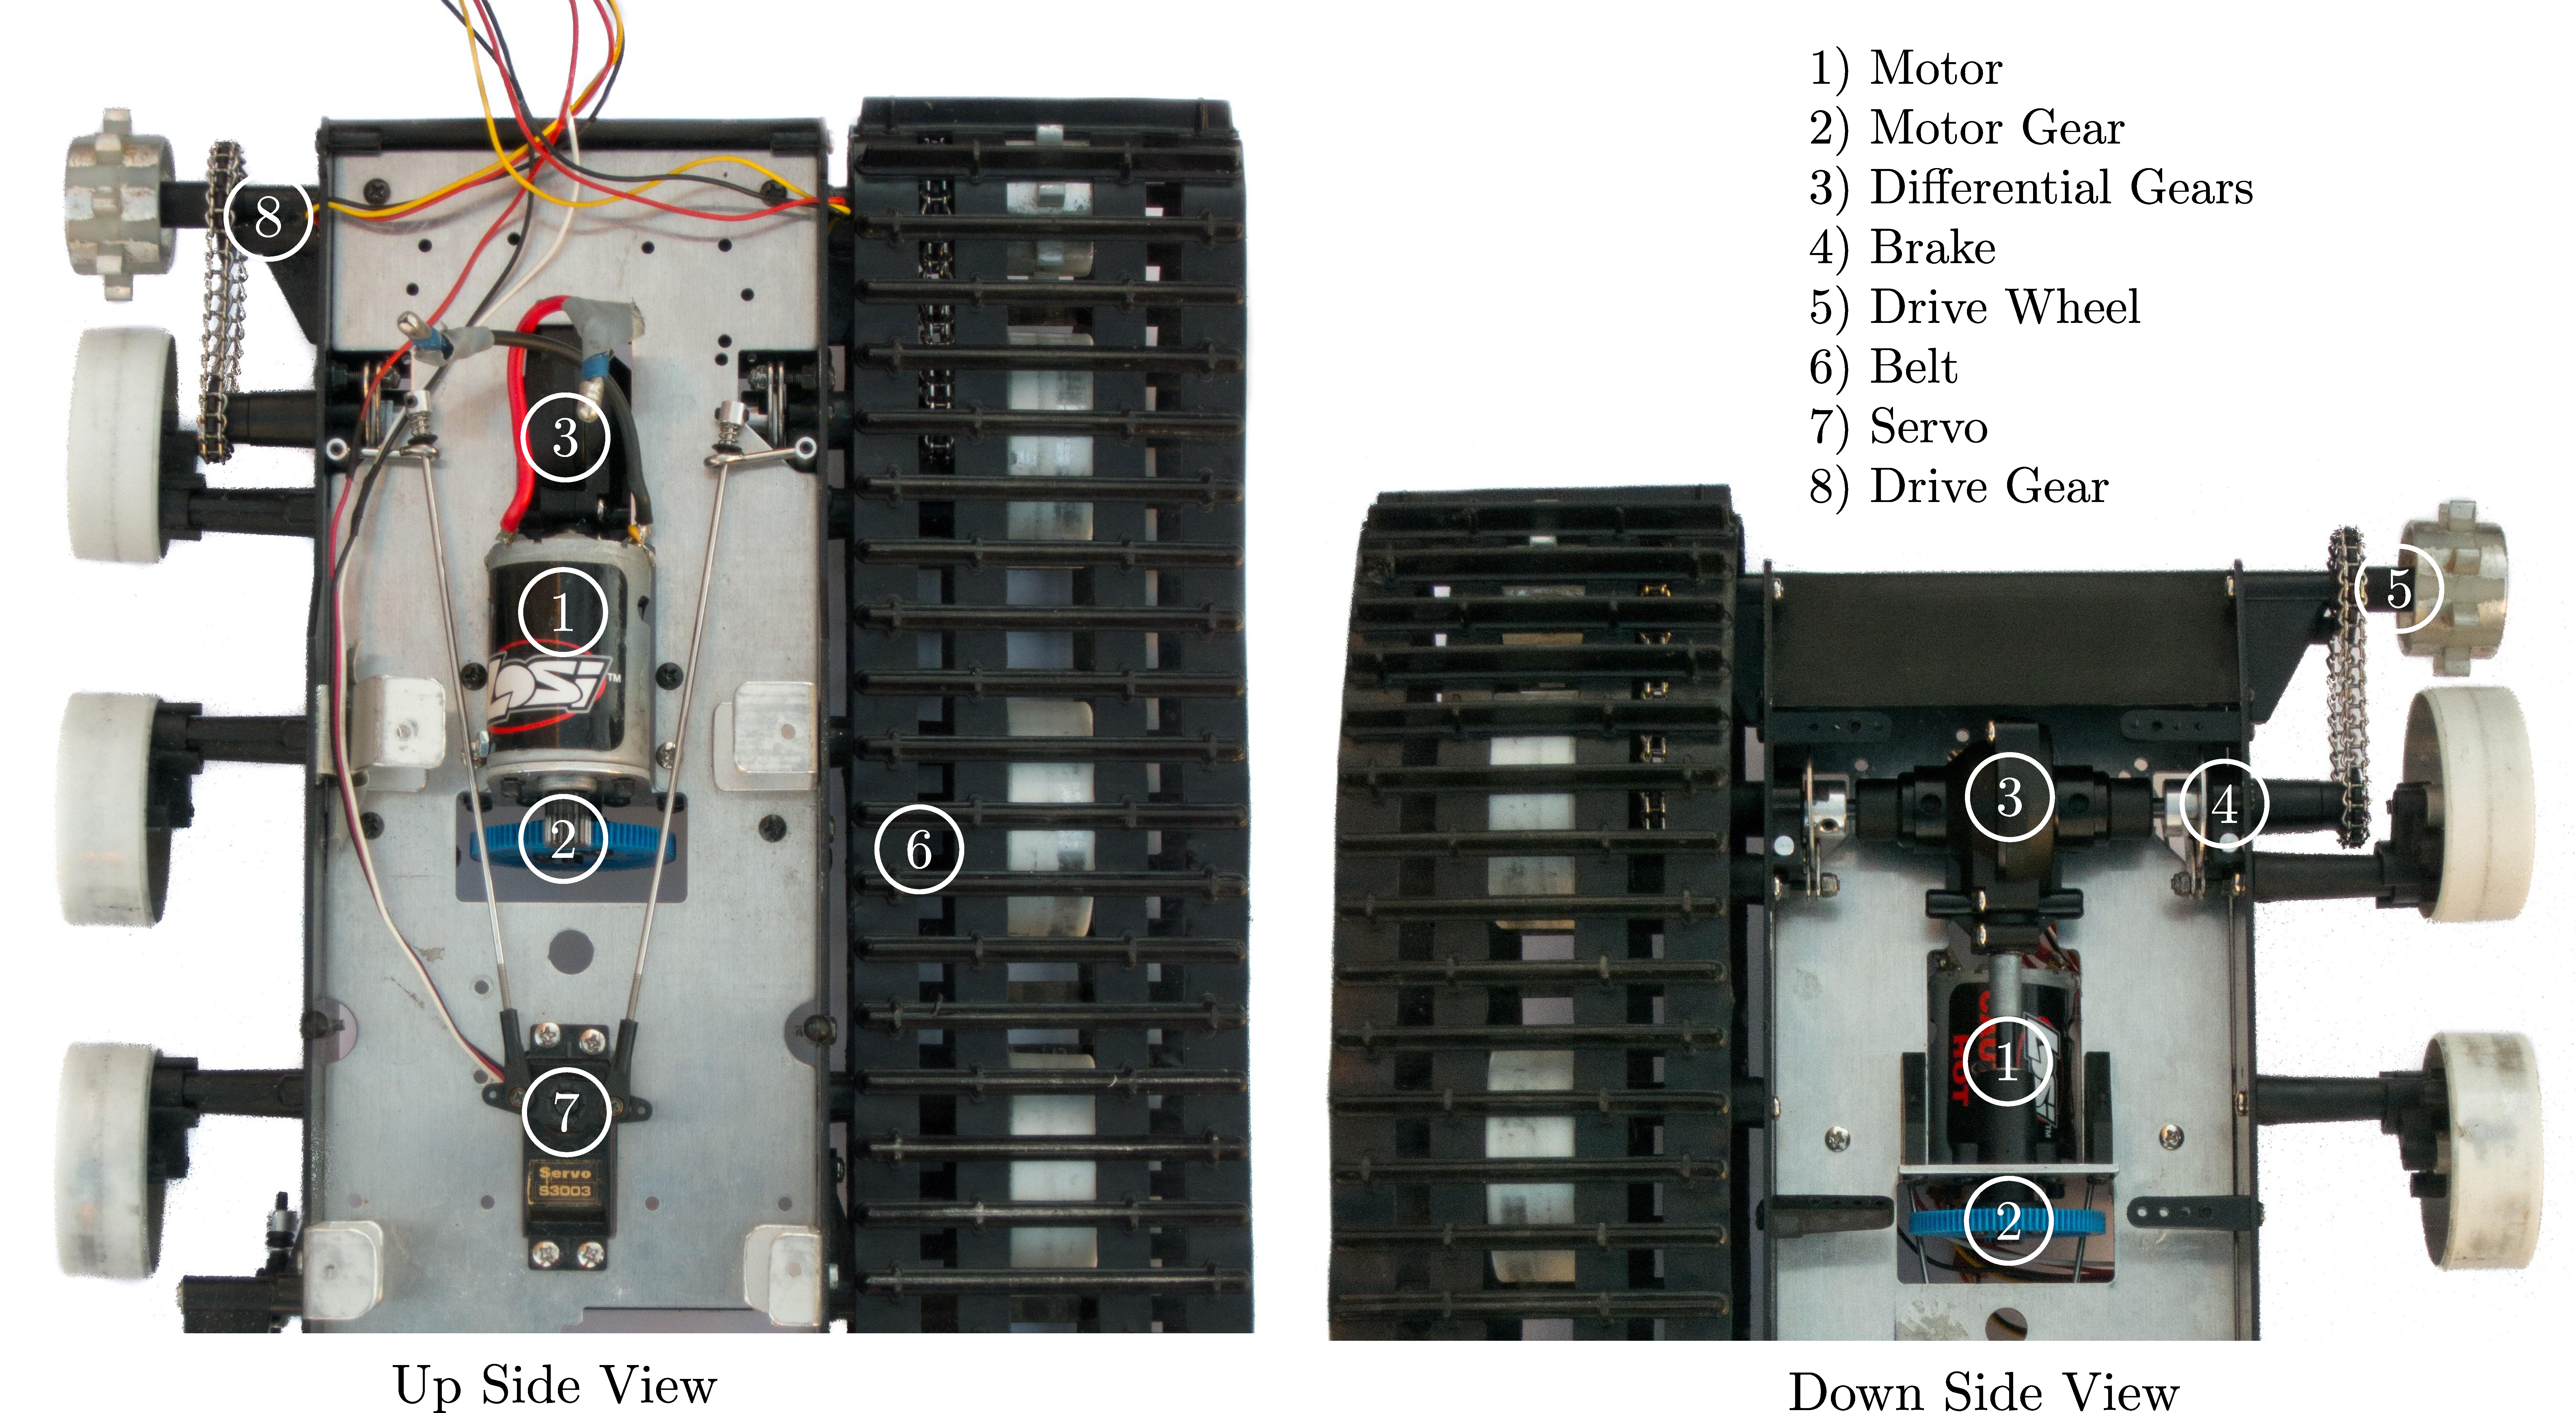
\includegraphics[scale=.09]{figures/FullVehicle.png}
	\caption{Picure presenting all the elements used on the vehicle.}
	\label{FullVehicle}
\end{figure}
%\noindent 1) Motor\\2)Motor Gear\\3)Differential Gears\\4) Brakes\\5) Drive Wheel\\6) Belts\\7) Servo

To model this vehicle, a simplified drawing of the vehicle is made. The drivetrain contains the gear connected to the brushed DC motor, the differential gear box and the gears connected to the belts. The drivetrain is illustrated in \figref{vehicleDescriptionDriveTrain}.

\begin{figure}[H]
	\centering
	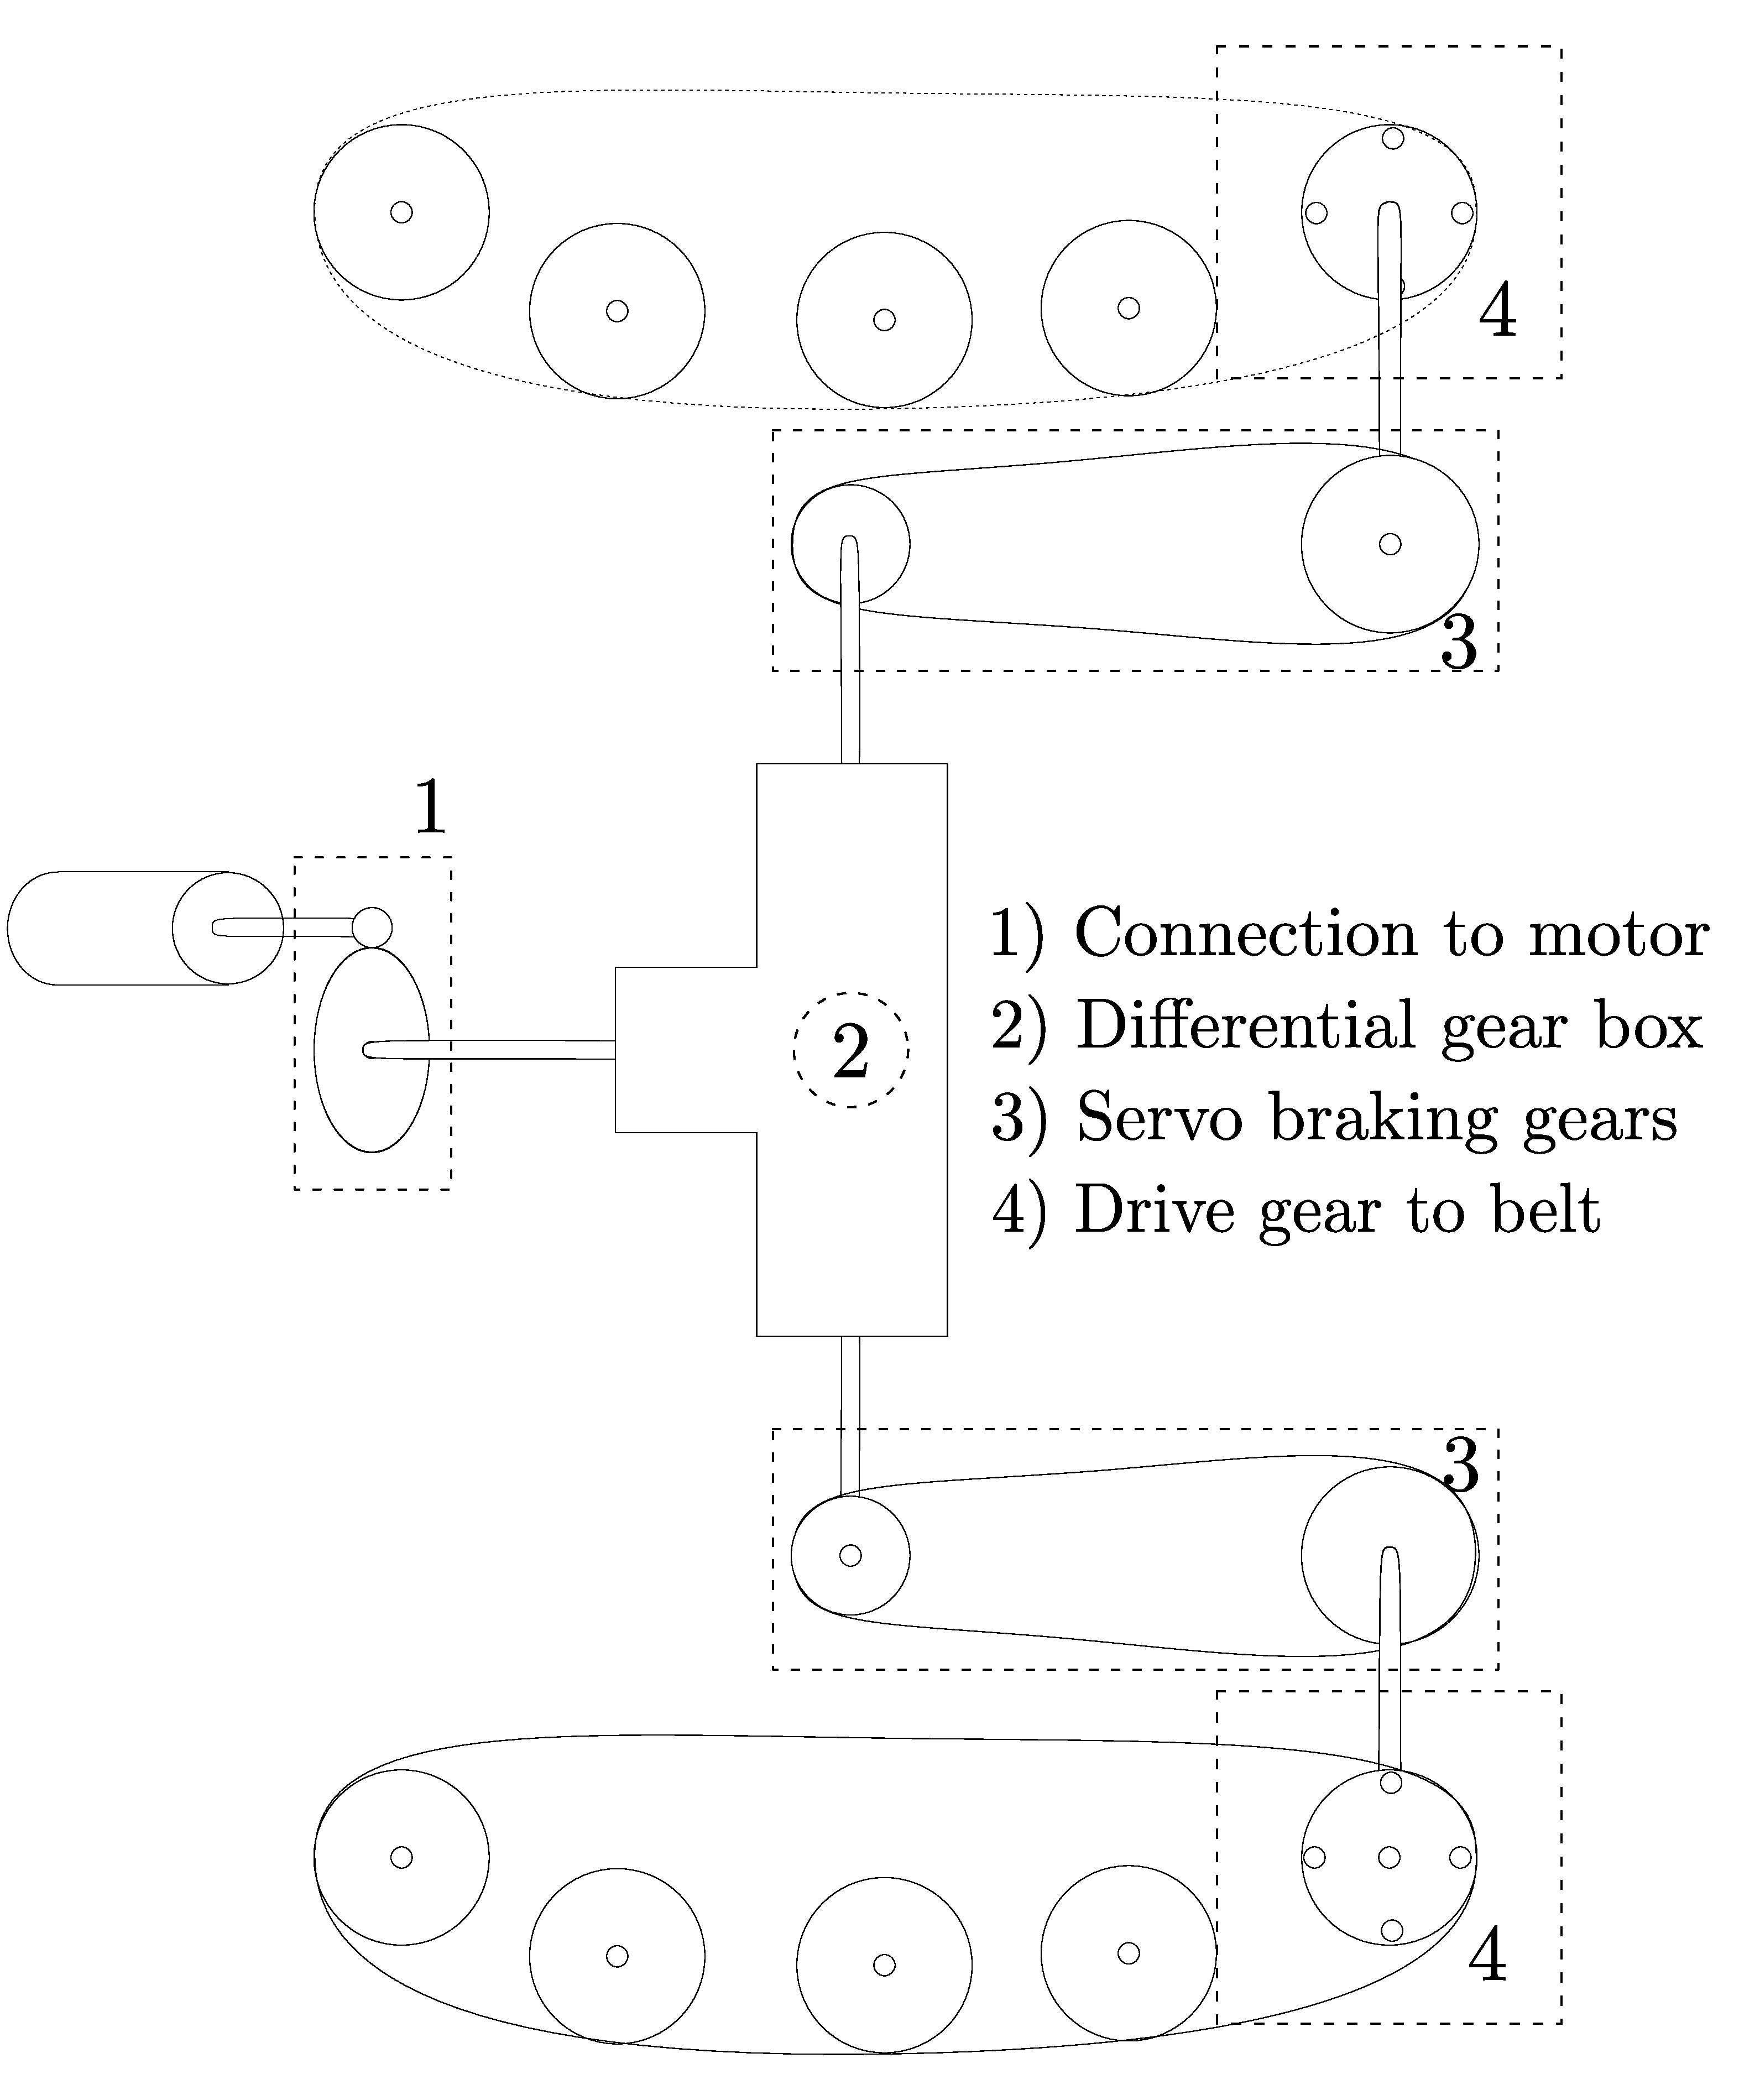
\includegraphics[scale=.25]{figures/vehicleDescriptionDriveTrain.pdf}
	\caption{Illustration of the drive train of the vehicle.}
	\label{vehicleDescriptionDriveTrain}
\end{figure}

In \figref{vehicleDescriptionDriveTrain} it can be seen that the motor delivers a force to the system through a the motor-shaft with a connecting gear. This gear is connected to the start of the drivetrain(1). From there the differential gear box is connected(2). From the differential gears two shafts are connected to a gear which transfers the velocity to the drive wheels(3).
From there the rotational velocity makes the drive-wheel turn, thus rotating the belts which are supported by four free wheels on each side(4). 

In the following segment, the differential gear box's function, seen in \figref{vehicleDescriptionDriveTrain}, is explained.